\section{Results}
\label{sec:results}

62 mechanical-turk trial results were analyzed, giving a total of 2480 moves.
For each move, the probability assigned by the particle filter to the
categorization decision made by the subject was recorded. The mean of these
$2480$ log probabilities was an unimpressive $-1379.256$, and the median was
$-29.612$.

The three histograms in figures \ref{fig:fullhist}, \ref{fig:smallhist}, and
\ref{fig:cumulativehist}, though, show that $48.9\%$ of the
log probabilities were greater than $-0.25$ and $51.5\%$ were greater than
$-1.0$. $1216$ moves saw the particle filter inference algorithm assigning
probabilities (\emph{not} log probabilites) greater than $0.5$ to the categorization selected by the human,
indicating that the particle filter model used in this experiment agreed with
the human data at least $49.032\%$ of the time. The average move involved a
choice between $4.929$ groups, making a $20.286\%$ success rate equivalent to
chance, and showing that the particle filter performed far better than chance.

\begin{figure}
\centering
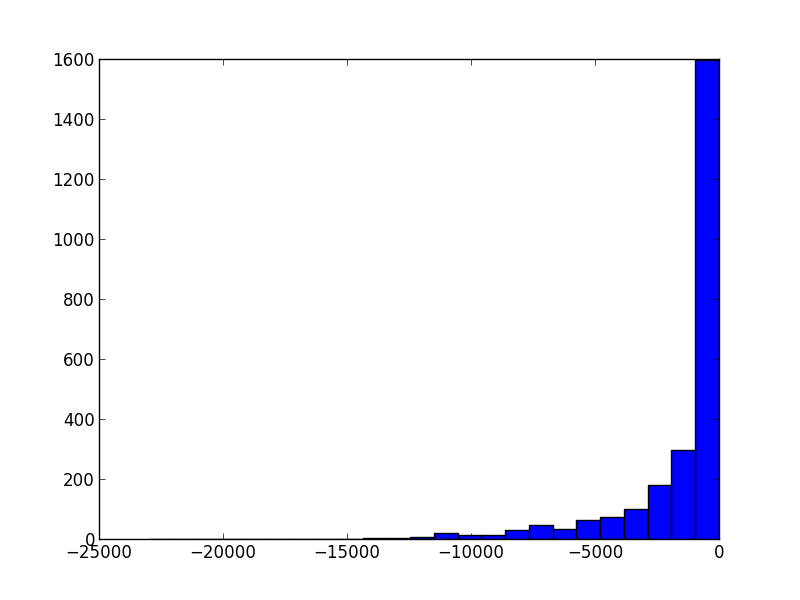
\includegraphics[scale=0.75]{img/hist0.png}
\caption{A histogram showing the log probability of the particle filter making
the same move as the human for each of the 2480 human moves.}
\label{fig:fullhist}
\end{figure}

\begin{figure}
\centering
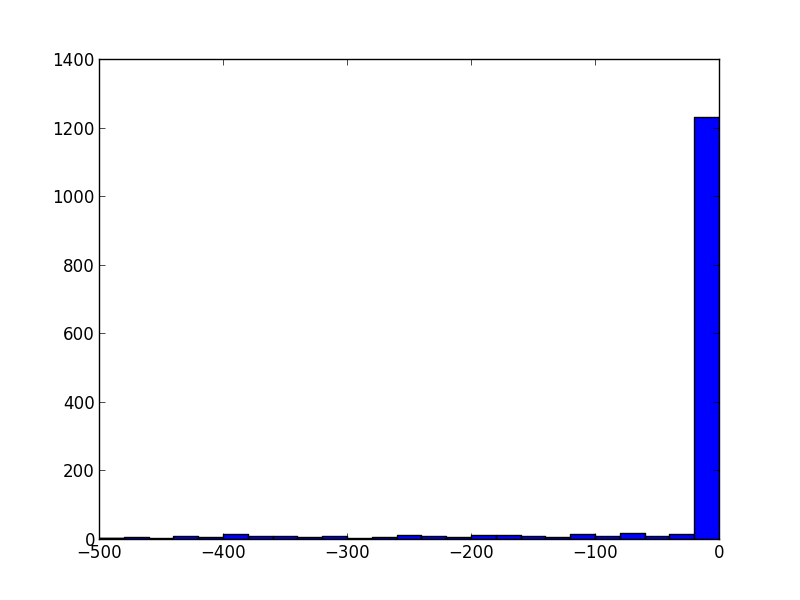
\includegraphics[scale=0.75]{img/hist4.png}
\caption{A histogram showing the log probability of the particle filter making
the same move as the human for each of the moves for which this value was
greater than $-500$. This is a zoomed in view, so to speak, of
\ref{fig:fullhist}.}
\label{fig:smallhist}
\end{figure}

\begin{figure}
\centering
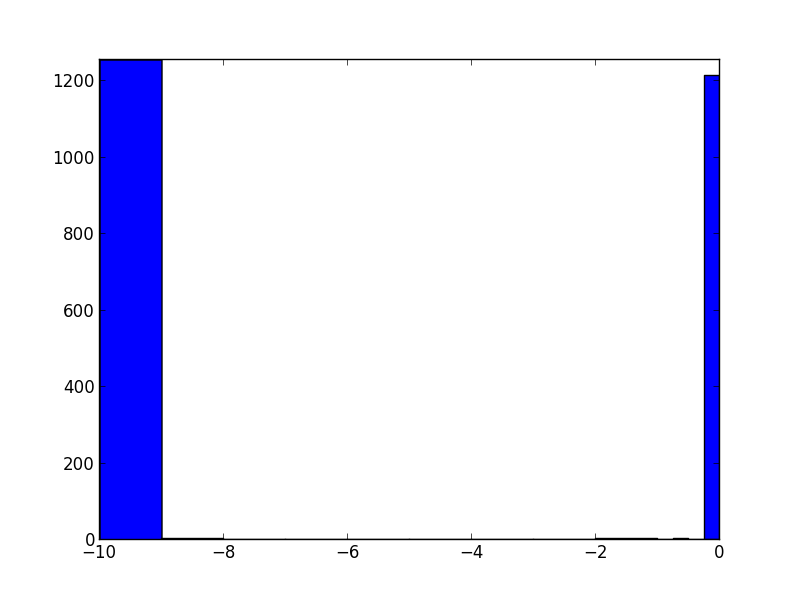
\includegraphics[scale=0.75]{img/hist8.png}
\caption{A histogram showing the log probability of the particle filter making
the same move as the human for each of the 2480 human moves, but with all moves
for which this value was less than $-9$ grouped into the lowest probability bin.}
\label{fig:cumulativehist}
\end{figure}

